%%%%%%%%%%%%%%%%%%%%%%%%%%%%%%%%%%%%%%%%%%%%%%%%%%%%%%%%%%%%%%%%%%%%%%%%%%%%%%%%
% Template for USENIX papers.
%
% History:
%
% - TEMPLATE for Usenix papers, specifically to meet requirements of
%   USENIX '05. originally a template for producing IEEE-format
%   articles using LaTeX. written by Matthew Ward, CS Department,
%   Worcester Polytechnic Institute. adapted by David Beazley for his
%   excellent SWIG paper in Proceedings, Tcl 96. turned into a
%   smartass generic template by De Clarke, with thanks to both the
%   above pioneers. Use at your own risk. Complaints to /dev/null.
%   Make it two column with no page numbering, default is 10 point.
%
% - Munged by Fred Douglis <douglis@research.att.com> 10/97 to
%   separate the .sty file from the LaTeX source template, so that
%   people can more easily include the .sty file into an existing
%   document. Also changed to more closely follow the style guidelines
%   as represented by the Word sample file.
%
% - Note that since 2010, USENIX does not require endnotes. If you
%   want foot of page notes, don't include the endnotes package in the
%   usepackage command, below.
% - This version uses the latex2e styles, not the very ancient 2.09
%   stuff.
%
% - Updated July 2018: Text block size changed from 6.5" to 7"
%
% - Updated Dec 2018 for ATC'19:
%
%   * Revised text to pass HotCRP's auto-formatting check, with
%     hotcrp.settings.submission_form.body_font_size=10pt, and
%     hotcrp.settings.submission_form.line_height=12pt
%
%   * Switched from \endnote-s to \footnote-s to match Usenix's policy.
%
%   * \section* => \begin{abstract} ... \end{abstract}
%
%   * Make template self-contained in terms of bibtex entires, to allow
%     this file to be compiled. (And changing refs style to 'plain'.)
%
%   * Make template self-contained in terms of figures, to
%     allow this file to be compiled. 
%
%   * Added packages for hyperref, embedding fonts, and improving
%     appearance.
%   
%   * Removed outdated text.
%
%%%%%%%%%%%%%%%%%%%%%%%%%%%%%%%%%%%%%%%%%%%%%%%%%%%%%%%%%%%%%%%%%%%%%%%%%%%%%%%%

\documentclass[letterpaper,twocolumn,10pt]{article}
\usepackage{usenix-2020-09}

% to be able to draw some self-contained figs
\usepackage{tikz}
\usepackage{amsmath}
\usepackage{amsfonts,amstext}

% necessary to depict some algorithms
\usepackage{algorithm,algpseudocode,float}
\usepackage{bbm}

% Let's suppress hbox warnings (https://tex.stackexchange.com/questions/138/what-are-underfull-hboxes-and-vboxes-and-how-can-i-get-rid-of-them)
\hbadness=99999

%-------------------------------------------------------------------------------
\begin{document}
%-------------------------------------------------------------------------------

%don't want date printed
\date{}

% make title bold and 14 pt font (Latex default is non-bold, 16 pt)
\title{\Large \bf ARMy Fuzzing - DRAFT}

%for single author (just remove % characters)
\author{
{\rm Andrew York}\\
Clemson University
\and
{\rm Kathryn Smith}\\
Clemson University
} % end author

\maketitle

%-------------------------------------------------------------------------------


%-------------------------------------------------------------------------------
% Input sections from other files
%-------------------------------------------------------------------------------
\section{Abstract}
%-------------------------------------------------------------------------------
Fuzzing is an easy and effective technique for testing software. As a result, 
many fuzzers have been developed, but one has not emerged as consistently superior. 
The growing number of available fuzzers has presented software developers with a 
selection burden.  To resolve this issue, Fu et al. developed \texttt{autofz}. 
\texttt{Autofz} is a dynamic fuzzer that seeks to maximize the bitmap coverage fuzzed
by deploying a set of fuzzers. During execution, each fuzzer is given resources 
proportional to preformance. This paper confirmed the effectiveness of \texttt{autofz} 
as proposed, expanded \texttt{autofz} for execution on ARM64 architectures, and introduced new
algorithms for evaluating the runtime performance of the individual fuzzers within 
\texttt{autofz}.
 %-------------------------------------------------------------------------------

%-------------------------------------------------------------------------------
\section{Introduction}
%-------------------------------------------------------------------------------

Due to the success of fuzzing as a method of identifying bugs in software, many fuzzers have been 
developed. Unfortunately, selecting a fuzzer is a difficult task. The following challenges prevent 
researchers from quickly selecting a fuzzer using benchmarking: no fuzzer consistently outperforms 
the others, the efficacy of a fuzzer is inconsistent throughout its execution, and fuzzing results 
are not reproducible.

In response to these problems, \texttt{autofz} was developed. \texttt{Autofz} leverages multiple fuzzers by dynamically 
allocating resources to fuzzers using runtime data. This methodology empowers \texttt{autofz} to eliminate the 
fuzzer selection problem and outperform individual fuzzers.

In spite of these successes, \texttt{autofz} is not perfect. While there is no consensus on the best way to 
assess fuzzers, \texttt{autofz} oversimplifies this process. \texttt{Autofz} originally relied on a 
singular metric, AFL bitmap coverage, to rank its fuzzers and allocate resources. In this paper, we
propose the use of unique bugs as an additional and alternative metric. We posit that, in 
many cases, \texttt{autofz} performs even better if it considers the number of unique bugs found when assigning 
resources to individual fuzzers.

Moreover, \texttt{autofz} prides itself on streamlining the fuzzer selection process for the novel user, but 
it was designed for and tested on a cluster of hosts, each boasting an AMD Ryzen 9 3900 with 24 cores 
and 32 GB memory. We believe that this is not representative of the standard user, and as a result, 
autofz needs to be adapted for use in additional environments. \cite{fu_autofz_2023} We posit that \texttt{autofz} can 
effectively deliver similar results on commodity, portable hardware (i.e. Apple MacOS based laptop 
computers) that is based on the ARM64 architecture. 

By investigating the implementation and results of \texttt{autofz} on this configuration, we identify some the 
challenges and opportunities presented by fuzzing on the ARM64 architecture.

In this effort, we seek to improve \texttt{autofz} and answer the following research questions:
\begin{itemize}
    \item \textbf{RQ1.} Can we successfully reproduce a working tool chain from
    Fu et al. \cite{fu_autofz_2023} on portable ARM64 computing devices?
    \item \textbf{RQ2.} Can we reproduce the results (e.g. number of defects found)
     of fuzzing at least two targets from Fu et al. \cite{fu_autofz_2023} on our ARM64-based
      tool chain?
    \item \textbf{RQ3.} \texttt{autofz} uses a single metric (i.e. AFL bitmap coverage) for
     allocation of resources to fuzzers. Can we identify at least one additional,
     alternate metric that will improve this allocation?
\end{itemize}

%-------------------------------------------------------------------------------
\section{Related Work}
%-------------------------------------------------------------------------------

\subsection{Fuzzing}
In 1990, Miller et al. proposed fuzz testing as a tool to identify bugs in Unix utilities and other 
applications. Their fuzzer generated, deployed and monitored the execution of random strings on a 
target program. The application could succeed, crash, or hang. The application was successful when 
program terminated normally, and the input did not identify a bug. Alternatively, if the input caused 
the program to crash or hang, a defect was discovered. Using this simple methodology, Miller et al. 
were able to uncover bugs within Unix utilities that had not been previously identified using formal 
testing procedures. \cite{miller_empirical_1990}

Since Miller et al. introduced fuzzing as an effective means of identifying bugs, over thirty more 
sophisticated fuzzers have been proposed. Most fuzzers conform to the basic methodology introduced by 
Miller et al; they generate test cases and deploy them on a target while monitoring its state. 

Despite their similarities, the test case generation phase varies between fuzzers. Fuzzers can be 
divided as generation-based or mutation-based fuzzers. Generation-based fuzzers generate inputs that 
conform with grammars while mutation-based fuzzers modify existing inputs. 

Fuzzers can also be divided into blackbox, whitebox, and greybox. Blackbox fuzzers only monitor the 
state of the target application before and after the execution of an input while whitebox fuzzers 
document the status of the target throughout execution, and greybox fuzzers monitor specific 
execution attributes. \cite{zhu_fuzzing_2022}

// add more detail about how seeds are generated

\subsection{Fuzzing Assessment Methods}
Despite the abundance of fuzzers and their differences in implementation and performance, a consensus
 has not emerged on how to compare them.

\subsubsection{AFL Bitmap Coverage}
Bitmap coverage is a one means of capturing a fuzzer's performance; it quantifies the number of
 branches explored by the fuzzer. To calculate bitmap coverage, instrumentation is injected at branch 
 points when the program is compiled. By marking these points in the binary, then the fuzzer can 
 identify which branches have and have not yet been taken during a fuzzing run. 
 \cite{noauthor_afldocstechnical_detailstxt_nodate}

 This coverage method was introduced in the American Fuzzy Lop (AFL) project \cite{noauthor_afldocstechnical_detailstxt_nodate}. 
 It is supported by fuzzers that are based on or otherwise derived from AFL.  AFL's developers 
 note that this approach makes distinguishing between different program traces trivial. It also draws 
 the fuzzer to the target's state transition points, where opportunities to enter undocumented states 
 are most likely. The bitmap is implemented as 64 kB of shared memory, or enough storage to 
 accommodate 65,536 coverage points, \emph{l} \cite{yun_qsym_2018}, each roughly implemented as:

 \begin{algorithm}
    \caption {Insert Bitmap}\label{bitmap}
    \begin{algorithmic}[1]
        \Procedure {Insert Bitmap}{$location$}$\ as\ b(l)$
            \State $l_{cur} \gets\ COMPILE\_TIME\_RANDOM$
            \State $b(l) \gets\ b[l_{cur}\  xor\  l_{prev}] + 1$
            \State $l_{prev} \gets\ l_{cur} >> 1$
        \EndProcedure
    \end{algorithmic}
\end{algorithm}
 
While using bitmap coverage allows competition amongst disparate fuzzers, this choice restricts the 
set of Autofz's supported fuzzers to those that implement AFL bitmap as a coverage metric. In algorithm 
\ref{bitmap}\, we define \emph{$l_{cur}$} as a random number that is assigned at compile time. While 
not implemented in our experiments, the bitmap metric can be implemented when testing black-box binaries; 
i.e. binary programs for which source code is not available to the tester. AFL (and some of its derivatives)
implements QEMU mode instrumentation \cite{noauthor_aflqemu_mode_nodate}, where bitmap composition is 
by \cite{noauthor_afldocstechnical_detailstxt_nodate}:

\begin{algorithm}
    \caption {Insert Bitmap, QEMU Mode}\label{qemu_bitmap}
    \begin{algorithmic}[1]
        \Procedure {Insert Bitmap}{$location$}$\ as\ b(l)$
          \If{$end_{elf_text} > addr_{block} > start_{elf_text}$}
                \State $l_{cur} \gets\ (addr_{block}\ >>\ 4)\ xor\ (addr_{block}\ <<\ 8)$
                \State $b(l) \gets\ b[l_{cur}\  xor\  l_{prev}] + 1$
                \State $l_{prev} \gets\ l_{cur} >> 1$
          \EndIf
        \EndProcedure
    \end{algorithmic}
\end{algorithm}

\subsubsection{Additional Metrics}
Ecezia et al. \cite{eceiza_improving_2023} asserted that the methodology for testing new and 
evaluating existing fuzzers needs to be standardized. In their proposed protocol, they 
recommended using three categories of metrics. They are bugs, coverage, and performance. 

\begin{itemize}
    \item \textbf{Bugs} Ecezia et al. recommends using the total number of
    bugs discovered as the best means of assessing the general performance 
    of a fuzzer. They argue that since number of bugs discovered 
    encompasses all other bug metrics, it is the superior bug metrics. 
    While total number of bugs identified may encompass unique bugs 
    discovered, unique bugs discovered is likely a better means of 
    measuring a fuzzers general performance. Total number of bugs 
    discovered includes duplicate bugs. This may result in a fuzzer that 
    discovers the few bugs many times appearing to perform better than 
    another fuzzer that discovers more unique bugs once. Moreover, once a 
    bug is known, it does not need to be discovered again.
    \item \textbf{Coverage} Coverage metrics communicate the performance 
    of a fuzzer's exploratory processes. While Ecezia et al. do not 
    explicitly identify bitmap coverage in their proposed method, they 
    recommend a combination of line and branch coverage for evaluating the 
    coverage achieved by a fuzzer. Despite this recommendation, they 
    maintain that complete line or branch coverage does not guarantee 
    complete bug discovery. Instead, they report that if the fuzzer does 
    not provide the target bug triggering input, an error may remain 
    undiscovered even after the buggy line of or path through code is 
    fuzzed. 
    \item \textbf{Performance} Performance metrics reflect the efficiency 
    of the fuzzer. Ecezia et al. reports that density is the best means of 
    measuring a fuzzer's efficiency. Density communicates the ratio of 
    number of tests completed to bugs discovered. A denser fuzzer will 
    need few runs to identify a bug, and consequently, identify more bugs 
    faster than a fuzzer with a lower density. 
\end{itemize}

\subsubsection{Experimental Conditions}
In addition to establishing the evaluation metrics, Ecezia et al. established  criteria for fuzzer 
test conditions. They asserted that in order to compare fuzzers, the fuzzers must be executed 
against the same applications, at least 15 times, and for the same period of time. These conditions 
are aimed at eliminating inconsistencies associated with evaluating fuzzers. 

For instance, fuzzers can only be compared if they are run on the same target application because 
the performance of a fuzzer is directly linked to the system under test. When a more buggy program 
is fuzzed, it will yield more bugs than a well-designed system regardless of the fuzzer. 

Moreover, when evaluating a fuzzer, it must be executed at least 15 times because the random input 
generated by a fuzzers will vary between runs.

The final condition that must be constant for each test is execution time; a fuzzer executed for 
10 hours cannot be compared to a fuzzer that has been running for 24 hours; the fuzzer that ran for 
24 hours will likely discover more bugs than the fuzzer that has run for 10 hours. The 24 hour fuzzer 
is not necessarily a better fuzzer, but it had more opportunities to discover unwanted behavior. 
\cite{eceiza_improving_2023}

\subsection{Autofz}
While Ecezia et al. looked to simplify the difficult task of identifying the best fuzzer by establishing 
evaluation criteria, Fu et al.\cite{fu_autofz_2023} aimed to eliminate the task. They proposed a new 
fuzzer that would make the task of evaluating and selecting an individual fuzzer obsolete. Autofz is a 
dynamic fuzzer that dynamically deploys a set of fuzzers. Autofz accomplishes this by dividing its 
workload into two phases; they are a preparation and a focus phase.

During the preparation phase, Autofz captures the runtime trends of multiple fuzzers on the target 
application. First, Autofz deploys the fuzzers with the same seeds. Each fuzzer executes for an equal 
portion of the preparation phase. Next, Autofz measures bitmap coverage achieved by each individual fuzzer. 
This process is repeated until the end of the preparation phase is reached or a strong trend emerges. A 
strong trend occurs when the difference in bitmap coverage of the best and worst performing fuzzer exceeds 
a predetermined threshold. 

Based on the data collected in the preparation phase, Autofz deploys the set of fuzzers with the potential 
to maximize the focus phase’s performance. More specifically, Autofz allocates resources to the fuzzers 
proportionally to their performance during the preparation phase. For example, the fuzzers that demonstrated 
the greatest bitmap coverage during the preparation phase have the most resources allocated to them during 
the focus phase, and the fuzzers that preformed poorly will have less available. This may result in one 
fuzzer receiving all available resources or no resources. After assigning resources to the individual fuzzers, 
the focus phase is executed. In the focus phase, each fuzzer is executed with its respective resources.

During the focus phase, Autofz achieved greater bitmap coverage than individual fuzzers that executed under 
the same conditions. \cite{fu_autofz_2023}

%-------------------------------------------------------------------------------
\section{Methodology}

% We need these declarations to use algorithms based on Fu et al.
\algblock{Input}{EndInput}
\algnotext{EndInput}
\algblock{Output}{EndOutput}
\algnotext{EndOutput}
\newcommand{\pdiff}{diff_{peak}}

%-------------------------------------------------------------------------------
In order to confirm the findings presented in Fu et.al.\cite{fu_autofz_2023}, we implemented our 
own instances of \texttt{autofz}. We implemented our evaluation environment by:

\begin{enumerate}
    \item Installing the containers provided by Fu et al. \cite{fu_autofz_2023} on our own
    AMD64 development workstation;
    \item Building our own containers, based on Fu et al. \cite{fu_autofz_2023} on our own
    AMD64 development workstation;
    \item Building our own containers, based on our own modifications to \texttt{autofz} on our own 
    ARM64 (Apple MacBook) laptop devices
\end{enumerate}

Moreover, we tested our implementations of \texttt{autofz} against the targets: exiv2, mp3gain, mojs, and 
tcpdump. Our initial findings validate the results presented in Fu et al.; \texttt{autofz} 
is consistently a top performing against the tested targets.

%-------------------------------------------------------------------------------
\subsection{Autofz on AMD64 - Validating Fu et al.\cite{fu_autofz_2023}}
%-------------------------------------------------------------------------------

To validate the results of Fu et al., we deployed a single physical workstation with 
an AMD FX\texttrademark - 6300 Six-Core Processor (3.5 GHz), 16 GB memory, and 1 TB 
SSD, running Ubuntu 20.04.6 LTS (focal). Containers were built on this host using 
the source code available at the sslab-gatech/autofz repository \cite{noauthor_sslab-gatechautofz_2024} 
and were also installed from fuyu0425/autofz images on docker hub\cite{noauthor_fuyu0425autofz_nodate}.


%-------------------------------------------------------------------------------
\subsection{Autofz on ARM64 - ARMy Fuzzing}
%-------------------------------------------------------------------------------

We have also been able to produce a working tool chain on ARM64, with some significant 
variations from Fu et al. \cite{fu_autofz_2023}. Our ARM64 environment supports 7 of 
the original fuzzers in Ubuntu 22.04 LTS. We configured these in virtual machines 
with the UTM app on host laptops running macOS 14.3.1 on Apple Silicon (ARM64) 
architecture \textbf{(RQ1)}. Key differences are described in Table \ref{arm64-characteristics}.

\begin{table}[ht]
    \begin{tabular}{|l|l|l|l|}
        \hline
                        & Original\cite{fu_autofz_2023} & ARM64 & Reason \\
        \hline
        Ubuntu Version  & 16.04             & 22.04 & 1 \\
        \hline
        aflforkserver.so    & x86\_64           & aarch64 & 2 \\
        \hline
        AFL (original)  & Yes               & Yes & \\
        \hline
        AFLFast         & Yes               & Yes & \\
        \hline
        Angora          & Yes               & No & 4 \\
        \hline
        Fairfuzz        & Yes               & Yes & \\
        \hline
        LAF-Intel       & Yes               & Yes & \\
        \hline
        LearnAFL        & Yes               & No & 3 \\
        \hline
        LibFuzzer       & Yes               & Yes & \\
        \hline
        QSYM            & Yes               & No & 4 \\
        \hline
        Radamsa         & Yes               & Yes & \\
        \hline
        RedQueen        & Yes               & Yes & \\
        \hline
    \end{tabular}
    \caption{Key differences between Original AMD64 and ARM64 Environments}
    \label{arm64-characteristics}
\end{table}

The majority of our changes were made in the \texttt{build.sh} scripts and \texttt{Dockerfile}s
for the affected containers.

There are a number of reasons for the differences between Fu et al.,
and our ARM64 environment. They correspond to the reason numbers in Table 
\ref{arm64-characteristics} and are:

\begin{enumerate}
    \item Ubuntu 16.04 LTS does not support the ARM64 architecture (also called 
    aarch64).
    \item Aflforkserver.so comes from the quickcov package, developed to support 
    the Cupid research project\cite{guler_cupid_2020}. We had to recompile it for aarch64.
    \item Learn AFL does not properly compile instrumented binaries for aarch64.
    \item Angora and QSYM are written such that they are dependent upon the x86\_64 ISA.
    They do not support other architectures.
\end{enumerate}

Our modified kit is published open-source and available on GitHub, 
\cite{noauthor_drewinchasautofz_nodate} placed in the arm64 branch 
of the drewinchas/autofz repository.

%-------------------------------------------------------------------------------
\subsection{An Additional Metric: Unique Bugs}
%-------------------------------------------------------------------------------

Fu et al.\cite{fu_autofz_2023} recognized that reliance on a single metric for resource 
allocation could potentially lead to unfair comparison with those fuzzers that do not 
utilize an edge coverage metric. Furthermore, our review of the original source 
code shows that \texttt{autofz} is not likely to produce meaningful improvements over individual 
fuzzers unless those individual fuzzers implement the AFL bitmap coverage metric.

We offer that the count of unique bugs discovered during \texttt{autofz}'s preparation phase 
as a useful, if not more universal metric \textbf{(RQ1)}. Eceiza et al.\cite{eceiza_improving_2023}'s 
survey of 36 fuzzers showed that the vast majority of them reported discovered 
bugs as a metric. To demonstrate and evaluate the use of this metric to inform resource allocation, we 
implemented a variation of the preparation phase as Algorithm \ref{prep-phase-with-ub}, 
where $\mathbb{UB}$ is the unique bugs metric.

%
% LaTex below comes from Fu et al.'s source code of their paper; modified for our purposes
%
\begin{algorithm}[h!]
  \caption{Preparation Phase, unique bugs (ub)}\label{prep-phase-with-ub}
  \small
  \begin{algorithmic}[1]
    \Output
      \State $Exit_{early} \gets$ Did preparation phase exit early?
      \State $T_{remain}$ $\gets$ Remaining time of preparation phase
    \EndOutput
    \Function{dynamic\_prep\_phase}{$\mathbb{F}$, $\mathbb{UB}$, $T_{prep}$, $1$, $C$}
      \State $T_{remain} \gets T_{prep}$
      \While {$T_{remain} > 0$}
        \State $T_{run} \gets min(T_{remain},30)$
        \If {$C == 1$}
          \For {\textbf{each} $f$ $\in$ $\mathbb{F}$}
            \State \Call{run\_fuzzer}{$f$, $T_{run}$}
          \EndFor
        \Else \Comment{multi-core implementation}
          \State \Call{run\_fuzzers\_parallel}{$\mathbb{F}$, $T_{run}$, $\frac{C}{|\mathbb{F}|}$}
        \EndIf
        \State $T_{remain} \gets T_{remain} - T_{run}$
        \State $diff_{peak} \gets $\Call{find\_most}{$\mathbb{UB}$}$ - $\Call{find\_least}{$\mathbb{UB}$}
        \If{$diff_{peak} \ge 1$}
          \State \Return $(Exit_{early}=True$, $T_{remain})$
        \EndIf
      \EndWhile
      \State \Return $(Exit_{early}=False, T_{remain})$
    \EndFunction
  \end{algorithmic}
\end{algorithm}

With the addition of this metric, we were able to implement two tie-breaker algorithms 
by combining the use of both metrics in the preparation phase. This is particularly 
useful when no unique bugs are discovered by any fuzzer during the preparation phase. 
In this case, we can use Algorithm \ref{prep-phase-with-ub-bitmap} to fall back to 
resource allocation by bitmap, where $\mathbb{B}$ is the bitmap metric and $\mathbb{UB}$ 
remains unique bugs.

\begin{algorithm}[h!]
  \caption{Preparation Phase: unique bugs (ub), then bitmap}\label{prep-phase-with-ub-bitmap}
  \small
  \begin{algorithmic}[1]
    \Output
      \State $Exit_{early} \gets$ Did preparation phase exit early?
      \State $T_{remain}$ $\gets$ Remaining time of preparation phase
    \EndOutput
    \Function{dynamic\_prep\_phase}{$\mathbb{F}$, $\mathbb{UB}$, $T_{prep}$, $\theta_{cur}$, $C$}
      \State $T_{remain} \gets T_{prep}$
      \While {$T_{remain} > 0$}
        \State $T_{run} \gets min(T_{remain},30)$
        \If {$C == 1$}
          \For {\textbf{each} $f$ $\in$ $\mathbb{F}$}
            \State \Call{run\_fuzzer}{$f$, $T_{run}$}
          \EndFor
        \Else \Comment{multi-core implementation}
          \State \Call{run\_fuzzers\_parallel}{$\mathbb{F}$, $T_{run}$, $\frac{C}{|\mathbb{F}|}$}
        \EndIf
        \State $T_{remain} \gets T_{remain} - T_{run}$
        \State $diff_{peak} \gets $\Call{find\_most}{$\mathbb{UB}$}$ - $\Call{find\_least}{$\mathbb{UB}$}
        \If{$diff_{peak} \ge 1$}
          \State \Return $(Exit_{early}=True$, $T_{remain})$
        \Else \Comment{fall back to bitmap}
          \State $diff_{peak} \gets $\Call{find\_best}{$\mathbb{B}$}$ - $\Call{find\_worst}{$\mathbb{B}$}
          \If{$diff_{peak} > \theta_{cur}$}
              \State \Return $(Exit_{early}=True$, $T_{remain})$
          \EndIf
        \EndIf
      \EndWhile
      \State \Return $(Exit_{early}=False, T_{remain})$
    \EndFunction
  \end{algorithmic}
\end{algorithm}

Conversely, we can fall back to the unique bugs metric as a tie-breaker as well. This is described in
Algorithm .

\begin{algorithm}[h!]
  \caption{Preparation Phase: bitmap, then unique bugs (ub)}\label{prep-phase-with-bitmap-ub}
  \small
  \begin{algorithmic}[1]
    \Output
      \State $Exit_{early} \gets$ Did preparation phase exit early?
      \State $T_{remain}$ $\gets$ Remaining time of preparation phase
    \EndOutput
    \Function{dynamic\_prep\_phase}{$\mathbb{F}$, $\mathbb{UB}$, $T_{prep}$, $\theta_{cur}$, $C$}
      \State $T_{remain} \gets T_{prep}$
      \While {$T_{remain} > 0$}
        \State $T_{run} \gets min(T_{remain},30)$
        \If {$C == 1$}
          \For {\textbf{each} $f$ $\in$ $\mathbb{F}$}
            \State \Call{run\_fuzzer}{$f$, $T_{run}$}
          \EndFor
        \Else \Comment{multi-core implementation}
          \State \Call{run\_fuzzers\_parallel}{$\mathbb{F}$, $T_{run}$, $\frac{C}{|\mathbb{F}|}$}
        \EndIf
        \State $T_{remain} \gets T_{remain} - T_{run}$
        \State $diff_{peak} \gets $\Call{find\_best}{$\mathbb{B}$}$ - $\Call{find\_worst}{$\mathbb{B}$}
        \If{$diff_{peak} > \theta_{cur}$}
          \State \Return $(Exit_{early}=True$, $T_{remain})$
        \Else \Comment{fall back to bitmap}
          \State $diff_{peak} \gets $\Call{find\_most}{$\mathbb{UB}$}$ - $\Call{find\_least}{$\mathbb{UB}$}
          \If{$diff_{peak} \ge 1$}
              \State \Return $(Exit_{early}=True$, $T_{remain})$
          \EndIf
        \EndIf
      \EndWhile
      \State \Return $(Exit_{early}=False, T_{remain})$
    \EndFunction
  \end{algorithmic}
\end{algorithm}

\textbf{Usage.} Implementation of these algorithms required some modifications to \texttt{autofz}'s 
command line interface, as well as modifications to the drawing program. When invoking 
autofz, the user may now specify \texttt{--discriminator bitmap | ub | ub-bitmap | bitmap-ub},
where:

\begin{itemize}
  \item \texttt{--discriminator bitmap} invokes \texttt{autofz} with AFL bitmap as the 
  fuzzer discriminator. This is the original \texttt{autofz} behavior. It is also the default behavior 
  when the \texttt{--discriminator} is not passed.
  \item \texttt{--discriminator ub} invokes \texttt{autofz} with unique bugs as discriminator. The 
  value for $\theta$ is ignored, as the discrimination threshold is fixed at 1, as described 
  in Algorithm \ref{prep-phase-with-ub}.
  \item \texttt{--discriminator ub-bitmap} invokes \texttt{autofz} with unique bugs as discriminator, 
  and bitmap as tie-breaker, as described in Algorithm \ref{prep-phase-with-ub-bitmap}.
  \item \texttt{--discriminator bitmap-ub} invokes autofx with bitmap as discriminator, 
  with unique bugs as tie-breaker, according to Algorithm \ref{prep-phase-with-bitmap-ub}.
\end{itemize}

Similarly, we modified the \texttt{autofz-draw} tool in order to create plots that 
differentiate between the new resource allocation algorithms. It now plots \texttt{autofz-bitmap}, 
\texttt{autofz-ub}, \texttt{autofz-ub-bitmap}, and \texttt{autofz-bitmap-ub}. In our 
implementation, \texttt{autofz-bitmap} is equivalent to the original \texttt{autofz}
%-------------------------------------------------------------------------------
\section{Findings}
%-------------------------------------------------------------------------------

Due to the time and resources available for our experiment, our efforts were limited 
to four targets, \texttt{exiv2}, \texttt{infotocap}, \texttt{mp3gain}, and 
\texttt{tcpdump}\textbf{(RQ2)}. Each of these were included in Fu et al.\cite{fu_autofz_2023} 
and are included in UNIFUZZ's\cite{li_unifuzz_2021} set of real-world programs for 
benchmarking fuzzers. As a baseline, UNIFUZZ's published counts of unique bugs are 
shown in figure \ref{fig:unifuzz_selections}.

\begin{figure}[h!]
    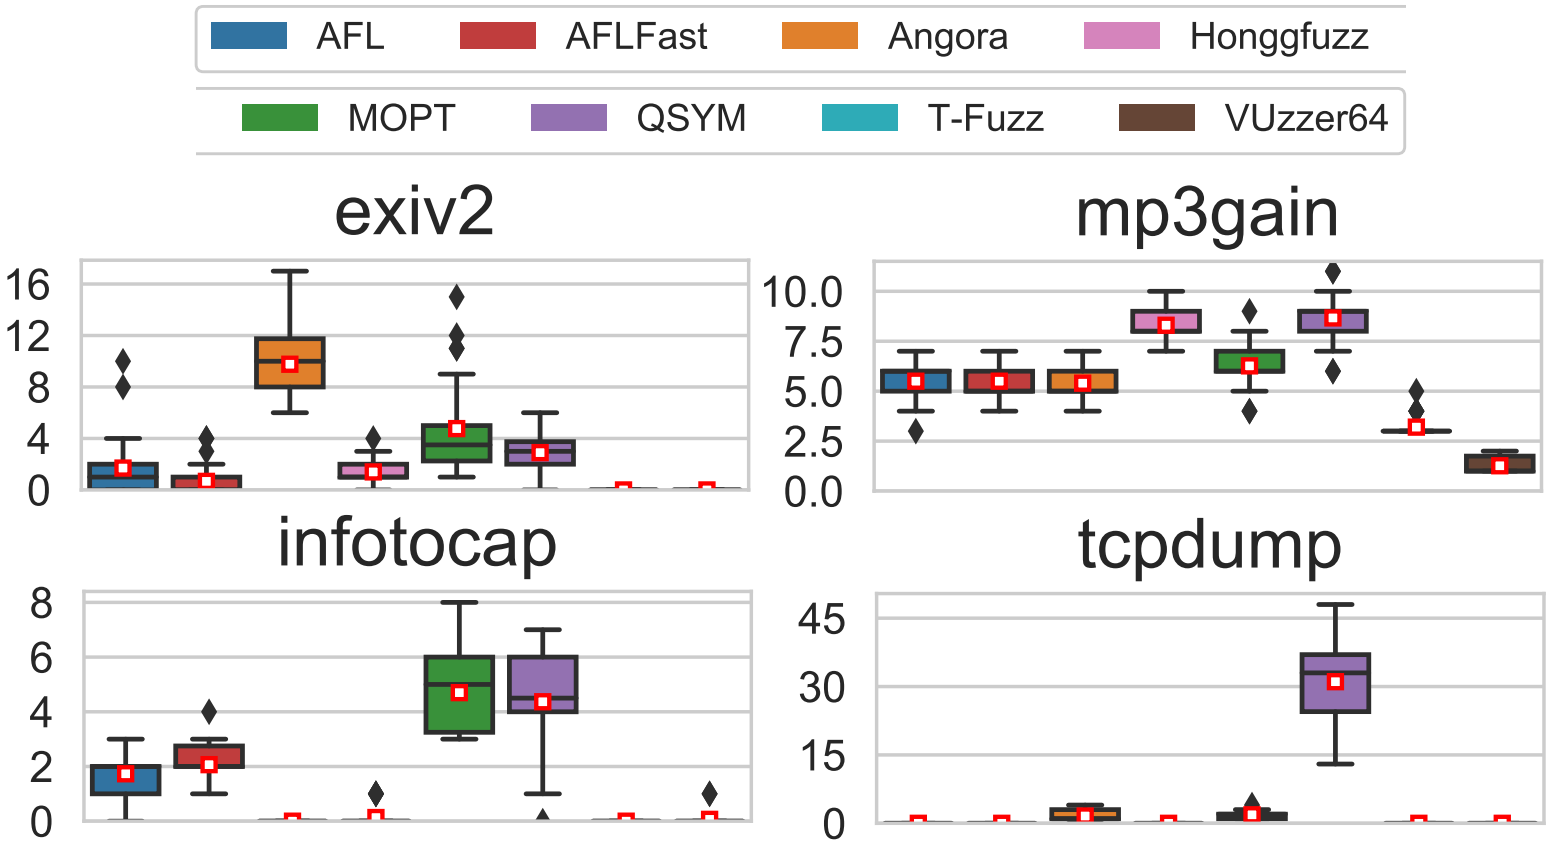
\includegraphics[width=0.5\textwidth]{figs/unifuzz_selections.png}
    \centering
    \caption{Counts of unique bugs found by the listed fuzzers, as documented in 
    UNIFUZZ\cite{li_unifuzz_2021}. These counts form the comparative baseline for 
    our work against Fu et al.\cite{fu_autofz_2023} and others.}
    \label{fig:unifuzz_selections}
\end{figure}

Figure \ref{fig:exiv2_compare_orig_arm64} displays bitmap density covered by the individual algorithms in our AMD64 implementation, 
as compared to a similar plot from Fu et al.\cite{fu_autofz_2023}. While our recreation of autofz achieved lower bitmap coverage than 
the version published by Fu et al., our individual fuzzers also achieved lower bitmap coverage. As a result, our replica still 
outperformed all other individual fuzzers tested in our environment. This is consistant
with Fu et al.'s findings and further proves that \texttt{autofz} is superior to individual fuzzers.

\begin{figure}
    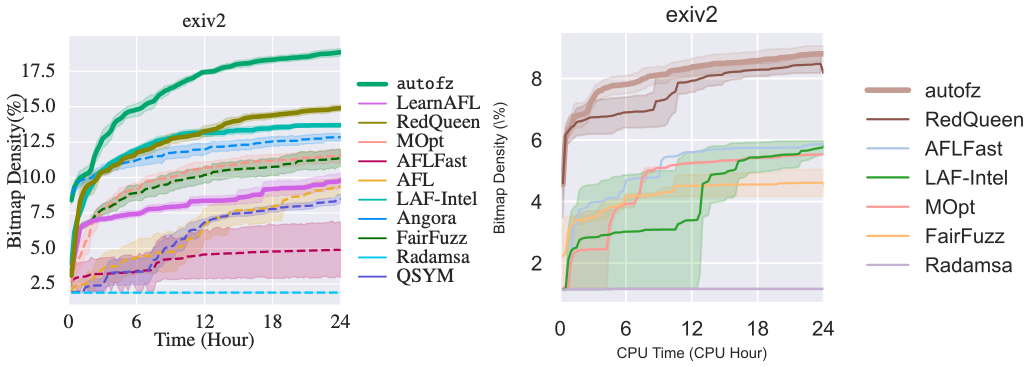
\includegraphics[width=0.52\textwidth]{figs/exiv2_compare_orig_arm64.png}
    \centering
    \caption{A comparison of bitmap density covered in the original\cite{fu_autofz_2023} and our 
    coverage during initial fuzzing of exiv2}
    \label{fig:exiv2_compare_orig_arm64}
\end{figure}

Testing also indicates that the ARM64 compatible \texttt{autofz} performs similarly to the unmodified AMD64 \texttt{autofz}. 
Bitmap density coverage of AMD64 \texttt{autofz} is plottted alogside our ARM64 \texttt{autofz} in figure 
\ref{fig:tcpdump_compare_orig_arm64}. After 24 hours, both implementations achieved similar bitmap coverage.
AMD64 \texttt{Autofz}'s bitmap coverage grew linearly while ARM64 \texttt{autofz} followed a logarithmic trend. Consequently, 
the AMD64 \texttt{autofz} took longer to achieve the same bitmap coverage. 

\begin{figure}
    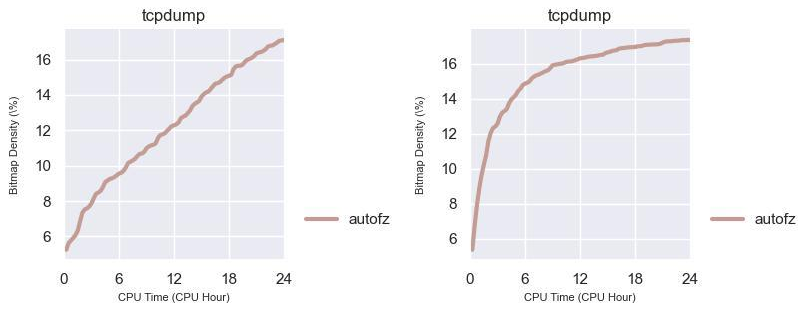
\includegraphics[width=0.52\textwidth]{figs/tcpdump_compare_orig_arm64.png}
    \centering
    \caption{A comparison of bitmap density covered in AMD64 \texttt{autofz} and our ARM64 implementation
    coverage during fuzzing of tcpdump}
    \label{fig:tcpdump_compare_orig_arm64}
\end{figure}

Bug coverage of our ARM64 fuzzing campaign against tcpdump is plotted in figure \ref{figs:tcp_compare_orig_arm64_ub.png}, 
shown as a comparison are results from Fu et al.\cite{fu_autofz_2023}. While the ARM64 adaptation of \texttt{autofz} achieved similar
performance to the original in bitmap coverage, it out performed the original in bug discovery. Since the other targets followed similar trends
when fuzzed with ARM64 \texttt{autofz}, \texttt{autofz} can be successfully adapted for the ARM64 architecture.

\begin{figure}
    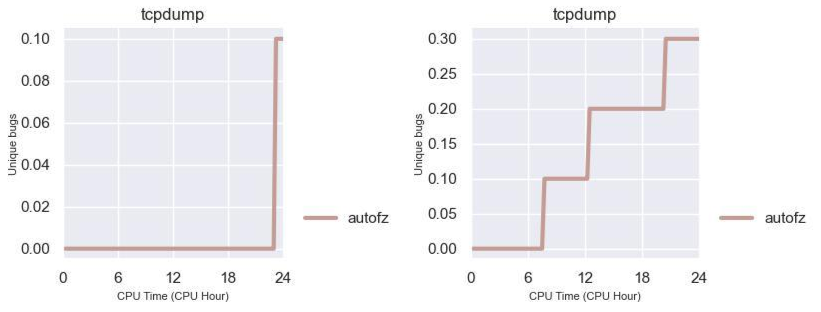
\includegraphics[width=0.52\textwidth]{figs/tcpdump_compare_orig_arm64_ub.png}
    \centering
    \caption{A comparison of bug discovery in AMD64 \texttt{autofz} and our ARM64 implementation
    coverage during fuzzing of tcpdump}
    \label{figs:tcp_compare_orig_arm64_ub.png}
\end{figure}

In addition to producing an ARM64 compatible \texttt{autofz}, we identified a potential improvement for \texttt{autofz}.
Existing versions of \texttt{autofz} use bitmap coverage to rank fuzzers during the preparation, but bitmap
coverage may not be the best metric for identifying the most effective fuzzers for a target. While
bitmap coverage indicates the portion of a target that was fuzzed, it does not guarantee bug discovery.
To resolve these problems, we plan to modify \texttt{autofz}, so fuzzers that discover more bugs during the
preparation phase are rewarded with more resources during the focus phase because discovering more bugs
across a smaller area of code decreases the attack surface by more entry points than discovering fewer
bugs over a greater area of the code.
%-------------------------------------------------------------------------------
\section{Future Research}
%-------------------------------------------------------------------------------
\subsection{Additional Targets} The version of \texttt{autofz} proposed by Fu et al. 
was tested against 12 targets and verified over 10 iterations. Our research  
confirmed the finding of Fu et al on 4 targets over ten repetitions. While we 
replicated the outcomes of Fu et al. with limited tests, the variations 
of \texttt{autofz} proposed in this paper need to under go additional testing. Due to their 
novelty, they cannot rely on previous literature to confirm their findings.

Similarly to \texttt{autofz}, we tested \texttt{autofz} for ARM64 against 4 targets over 10 
iterations. While trends were able to be identity among the tested targets, this
sample is not large enough to apply the outcomes to all targets. 

Additionally, the proposed algorithms for resources allocation during the preparation
underwent restricted testing, and they were insconsistant between targets. 
More testing needs to be undertaken in order to confirm the performance on tested targets and
extrapolate their performance to untested targets.

\subsection{Complex Targets} All versions of \texttt{autofz} need to be tested against 
complex targets. Fu et al. evaluated \texttt{autofz} against simple targets with known bugs. In 
order to compare our findings to Fu et al., we were restricted to testing our 
iterations of \texttt{autofz} against the same targets. In the future, all variations of 
\texttt{autofz} should be tested against larger, more complex targets that are comparable to
targets that may leverage fuzzing.

\subsection{Fuzzer Pool Composition} Fu et al. disclosed that the performance of
Autofz is dependent of the composition of its fuzzer pool. When \texttt{autofz} was presented
with a large pool of fuzzers and when \texttt{autofz} was provided with too few fuzzers, it 
under preformed. Further testing needs to be undertaken in order to determine the ideal
number of fuzzer in the pool as well as which fuzzers should be in the pool.

\subsection{Documentation} In addition to confirming and maximizing the performace of \texttt{autofz},
\texttt{autofz} needs undergo additional documentation. In route of evaluating \texttt{autofz}, significant 
changes were made to its graphing function. While these simplified comparing the performance of the variations
of \texttt{autofz}, they did not improve the performance of \texttt{autofz} and were outside of the scope of our research.
As a result, these modifications were not documented and need to testing. 





%-------------------------------------------------------------------------------

\bibliographystyle{plain}
\bibliography{output}

%%%%%%%%%%%%%%%%%%%%%%%%%%%%%%%%%%%%%%%%%%%%%%%%%%%%%%%%%%%%%%%%%%%%%%%%%%%%%%%%
\end{document}
%%%%%%%%%%%%%%%%%%%%%%%%%%%%%%%%%%%%%%%%%%%%%%%%%%%%%%%%%%%%%%%%%%%%%%%%%%%%%%%%

%%  LocalWords:  endnotes includegraphics fread ptr nobj noindent
%%  LocalWords:  pdflatex acks
